
When estimating an uncertain quantity it is natural to seek to minimize the error we commit. One natural way to quantify the error incurred by an estimator is to evaluate the squared deviation of the estimate from the true value. We can then take the average of this error over multiple realizations of the signal process or over a long time realization of it to obtain an estimate of the average error incurred by our estimator. This is the mean squared error\marginnote{Mean Squared Error $\equiv$ MSE} of the estimator and we can write generally
\[
MSE(\hat{X}) = \boldsymbol{E}\left[ (\hat{X} - X)^\top (\hat{X}-X)\right].
\]
Note that we can consider the average to be over the data distribution, over different repetitions of the experiment, over a long time realization of the signal process or further to be an ensemble average over all possible realizations of a process according to some model of its distribution. If we further know that our estimator depends on some parameters $\theta$, we could seek out the optimal estimator $\hat{X}^*$ by taking the parameters $\theta^*$ which minimize the MSE
\[
\theta^* = \textrm{argmin}_\theta MSE( \hat{X}(\theta)  ).
\]
Note that assuming we are estimating $X$ from an observation process $Y$ dependent on $X$, we can write
\begin{equation}
\label{eq:bayes_mse}
MSE( \hat{X}(Y) ) = \int dX dY  (\hat{X}(Y) - X)^\top (\hat{X}(Y)-X) P(X|Y)P(Y).
\end{equation}
Note that, since $P(Y)\ge 0$ for every $Y$, we know that minimizing the inner integrand $\int dX (\hat{X}(Y) - X)^\top (\hat{X}(Y)-X) P(X|Y)$ for every $Y$ will lead to a minimum of the full integral. We can then proceed to minimizing the inner integrand by simply taking a derivative of it with respect to the estimator. This will lead to
\[
\frac{\partial \int dX (\hat{X}(Y) - X)^\top (\hat{X}(Y)-X) P(X|Y)}{\partial \hat{X}(Y)} = 2 \int dX (\hat{X}(Y) - X) P(X|Y).
\]
Equating the derivative to zero we will obtain the Bayes estimator for $X$, given by
\[
\hat{X}^*(Y) = \int dX\, X\, P(X|Y) = \boldsymbol{E}[X|Y].
\]
Thus, the Bayes estimator minimizes the expected MSE as defined in \fref{eq:bayes_mse}. Note, however, that the optimal estimator can only be exactly computed if we know the true data generating distribution $P(Y|X)$, along with the true signal distribution $P(X)$. Furthermore, the Bayes estimator involves averaging over the signal space, which can be often impractical. This is, nevertheless, a central result in information theory, and the Bayes estimator is usually taken as the golden standard to estimation.\par
Note that, however, finding the optimal Bayes estimator is not the end of the story. Often the design of sensors and of the experimental process allows us to change the data generating distribution $P(Y|X)$. For a simple example, let us consider a radar gun. Assume it gives us a measure of the speed of the considered vehicle corrupted  with Gaussian noise with zero mean and standard deviation of $5\,\textrm{km/h}$. Indeed, if we are given a number of measurements of the speed of a vehicle\marginnote{Assuming the speed of the vehicle remained unchanged across measurement}, the Bayes estimator will be the estimator which minimizes the expected MSE. Regardless of that, however, we can always reduce our MSE by using a radar gun with a smaller noise rate. If we find a superior radar gun which outputs measurements with standard deviation of $1\,\textrm{km/h}$, this will certainly reduce our MSE further. In most simple cases, however, this reduction is trivial, as one simply strives to reduce the noise as much as possible.\par
The neural case poses an interesting exception though. If we consider the Poisson model from the previous chapter, the probability of a spike being fired in a small time interval $dt$ conditioned on the stimulus $X$ is given simply by $\lambda(X)dt$. The probability of a spike being fired would then be given by $\hat{\lambda}dt = \int dX\, P(X)\, \lambda(X)dt$. Note now, that if we try to increase the precision of the likelihood defined by $\lambda(X)$, for example by reducing the width of the tuning function, we will automatically reduce the probability of that neuron firing. Therefore, there is a trade-off between frequency of firing and precision of firing, which is not present in the case of additive Gaussian noise.

\section{The MSE for Dense Gaussian DSPP Observations}

The case discussed in \fref{sec:fast_coding} allows for a number of simplifications. Since the posterior Bayesian estimator is optimal in the MSE sense, its MSE will be the minimal Mean-Squared-Error attainable by an estimator.\marginnote{Minimal Mean-Squared-Error$\equiv$MMSE. Jeez!} We will then have, using the same notation as in \fref{sec:fast_coding}
\[
MMSE(t;\{\theta_i\},A) = \boldsymbol{E}\left[\left(X(t) - \hat{X}(\boldsymbol{N}_{[t_0:t]})\right)\left(X(t) - \hat{X}(\boldsymbol{N}_{[t_0:t]})\right)^\top\middle| X, \boldsymbol{N}\right]\equiv \epsilon(t).
\]
Note that we are here interested in the ensemble average over all possible realizations of both the signal as the observation processes. It is already established that the estimator $\hat{X}(\boldsymbol{N}_{[t_0:t]} = \boldsymbol{E}\left(X(t)\middle|\boldsymbol{N}_{[t_0:t]}\right)$ is the optimal estimator, but we can still improve that estimator by adapting the parameters of our encoding processes $\boldsymbol{N}$, more specifically the tuning covariance $A$. Assuming that our knowledge of the system's parameters is correct, we can evaluate part of the average exactly. Let us break up the expectation over $X$ and $\boldsymbol{N}$ as
\[
\epsilon(t) = \int d\mu(X) \int d\mu(\boldsymbol{N}_{[t_0:t]}) \left(X(t) - \hat{X}(\boldsymbol{N}_{[t_0:t]})\right)\left(X(t) - \hat{X}(\boldsymbol{N}_{[t_0:t]})\right)^\top P(X| \boldsymbol{N}_{[t_0:t]}) P(\boldsymbol{N}_{[t_0:t]}).
\]
Note that the average over $P(X|\boldsymbol{N}_{[t_0:t]})$ will just yield the posterior variance $\Sigma(\boldsymbol{N}_{[t_0:t]})$. We will then have simply
\[
\epsilon(t) = \boldsymbol{E}\left[\Sigma(\boldsymbol{N}_{[t_0:t]})\right] = \boldsymbol{E}\left[\Sigma(N_{[t_0:t]})\right],
\]
where in the last step we have used that the posterior variance is only a function of the spike count $N_{[t_0:t]} = \sum_i N^i_{[t_0:t]}$ and not of the full spike train $\boldsymbol{N}_{[t_0:t]} = \left(N^1_{[t_0:t]}, N^2_{[t_0:t]}, \ldots\right)^\top$. This makes it much simpler to treat the averages, but they still remain intractable. To get a sense of the problem, for every possible spike count, we would have to average over all possible spike times for those spikes, considering the evolution of $\Sigma$ from its initial value according to the dynamics given in \fref{eq:filtering_sde_sigma}, and then average over all possible spike counts. This has been done for the case of static stimuli in \citet{Yaeli2010}. When the stimulus is static, the averages are simplified by the fact that the variance does not change between spikes. The posterior variance is then simply given by
\[
\Sigma(t) = \left(\Sigma(t_0)^{-1} + N(t) A^\dagger\right)^{-1}.
\]
Averaging over the spike trains then amounts to averaging over all possible spike counts for the given time period. This will lead to
\begin{equation}
\epsilon_{static}(t) = \sum_{k=0}^\infty  \left(\Sigma(t_0)^{-1} + k A^\dagger\right)^{-1} \frac{ (\hat{\lambda}t)^k e^{-\hat{\lambda} t }}{k!}.
\end{equation}
Note that this simplifies further when $A = \Sigma(t_0)$, that is, when the tuning is matched to the prior variance of the static process. We will then have
\begin{equation}
\epsilon_{static}(t) =\Sigma(t_0)e^{-\hat{\lambda} t}  \sum_{k=0}^\infty  \frac{ (\hat{\lambda}t)^k }{(k+1)!} = \Sigma(t_0) \frac{1-e^{-\hat{\lambda} t }}{\hat{\lambda} t}.
\end{equation}
In the general case, the infinite sum has to be evaluated numerically. This case has been discussed extensively by \citet{Yaeli2010}, and a similar treatment of finite state continuous time systems has been considered in \citet{Bobrowski2009}.\par
When considering the general case, though the average can not be evaluated explicitly. One way to overcome this is to look at the evolution of $\epsilon(t)$ over time. Note that the posterior variance process is a simple drift-jump process with a constant jump rate. The evolution of the probability $P(\Sigma(t) = s | \Sigma(t_0) = s_0) \equiv P(s,t)$ is given by the differential Chapman-Kolmogorov equation\cite{Gardiner2004}
\begin{equation}
\label{eq:sigma_DCKE}
\frac{\partial P(s,t)}{\partial t} = -\nabla \left[B(s) P(s,t)\right] + \hat{\lambda} C(s) P\left( (s^{-1} - A^+)^{-1},t\right) - \hat{\lambda} P(s,t),
\end{equation}
where $B(s) = G s + s G^\top + \sigma$, and  $C(s) = 1/|\det(J(s))|$, where $J(s)$ is the Jacobian matrix
\[
J_{(i,j),(k,l)} = \frac{\partial (s^{-1}+A^+)^{-1}_{i,j}}{\partial s_{k,l}} = (I+A^+s)^{-1}_{k,i}(I+s A^+)^{-1}_{j,n}.
\]
Note that the exact order in which we choose to write up the Jacobian matrix does not matter as it would only account for a change in sign of the determinant, which only enters into \fref{eq:sigma_DCKE} through its absolute value. The differential Chapman-Kolmogorov equation is a generalization of the Focker-Planck and Kolmogorov forward equation to systems with drift, diffusion and jumps. We can use it to easily to evaluate the evolution of averages over $s$ by noting that
\[
\frac{\partial \int d\mu(s) P(s,t) f(s)}{\partial t} = \int d\mu(s) \frac{\partial P(s,t)}{\partial t} f(s),
\]
and assuming that $\lim_{s_{i,j} \to \infty} P(s,t) f(s) = 0$ for any $(i,j)$, we have that
\[
\frac{\partial \left<f(s)\right>}{\partial t} = \int d\mu(s) \left[\nabla f(s) B(s) P(s,t) - \lambda C(s) f(s) \left(P((s^{-1} + A^\dagger)^{-1},t)  -P(s,t)\right)\right].
\]
We can then obtain the evolution of our MMSE by taking $f(s) = s$, yielding
\begin{equation}
\label{eq:epsilon_exact}
\frac{d\epsilon(t)}{dt} = G\epsilon(t) + \epsilon(t) G^\top + \sigma -\hat{\lambda} \boldsymbol{E}\left[s (s+A)^{-1} s\right].
\end{equation}
Note that we are still left with the far right hand term, which involves a nonlinear average over the distribution of variances. There are many ways to deal with that. One is to approximate the distribution $P(s,t)$ by some parametric distribution and obtain an approximation for the evolution of $\epsilon(t)$. Another possibility is to evaluate the average numerically by sampling from the paths of \fref{eq:filtering_sde_sigma}. Another popular alternative is to approximate the distribution $P(s,t)$ by a point mass at its mean. This is the so-called Mean-Field approach, where we simply disregard all fluctuations in $s$ and approximate all averages $\boldsymbol{E}[f(s)]$ by $f(\boldsymbol{E}[s])$. This would lead to the mean-field evolution of $\epsilon(t)$
\begin{equation}
\frac{d\epsilon(t)}{dt} = G\epsilon(t) + \epsilon(t) G^\top + \sigma -\hat{\lambda} \,\epsilon(t) \left(\epsilon(t)+A\right)^{-1} \epsilon(t).
\end{equation}
The mean-field and sampling approaches are compared in \fref{fig:matern_coding}. As we can see, the mean-field approximation yields extremely good results, for the equilibrium and relaxation behavior of $\epsilon(t)$.\par
Although we can in principle evaluate the temporal evolution of the MSE, one must note that if we are seeking to optimize our encoder with respect to it, that will be of little use, as we seek a scalar measure of the quality of our encoder. We can however, still decide as to how we will measure the quality of our temporal estimator. The simplest idea is to simply take the long-time equilibrium value of the MSE as our measure. This would mean we are looking at the equilibrium MSE, give by
\[
\epsilon_{eq} = \lim_{t\to\infty} \epsilon(t).
\]
Another option would be to consider the time average of the MSE over a period specified by some experimental requirement. This would give us
\[
\epsilon_{T}\left(\Sigma(t_0)\right) = \int_{t_0}^T \epsilon(t) dt.
\]
Note that this is not as simple a measure, as it still depends on the prior variance $\Sigma(t_0)$. One way to do away with that is to take the limit of the average when $T\to\infty$. This would lead another equilibrium measure, which for ergodic systems should not depend on the initial variance anymore, yielding our long time limit
\[
\epsilon_{lt} = \lim_{T\to\infty}\epsilon_T \left(\Sigma(t_0)\right).
\]
This should be essentially equal to the equilibrium MSE defined above, however, and we will concentrate on that from now on.
\par
\subsection{Optimal Encoder for the One-Dimensional OU Process}
I will now consider a simple case of stochastic process, which will provide further insight to our analysis. We will look at the one-dimensional Ornstein-Uhlenbeck process, given by
\[
dX_t = -\gamma X_t dt + \sigma^{1/2} dW_t.
\]
Since the stimulus is one-dimensional, our tuning matrix has only one entry, which we will here call $\alpha$. The intensity functions are then given by
\[
\lambda ^i(x) = \phi \exp\left(-\frac{(\theta_i-x)^2}{2\alpha^2}\right).
\]
\Fref{eq:epsilon_exact} will then simplify to
\begin{equation}
\label{eq:epsilon_1d_exact}
\frac{d\epsilon(t)}{dt} = -2\gamma \epsilon(t) + \sigma -\hat{\lambda} \boldsymbol{E}\left[\frac{s^2}{\alpha^2+s}\right].
\end{equation}
The mean-field approximation is then given by
\begin{equation}
\label{eq:epsilon_1d_mf}
\frac{d\epsilon(t)}{dt} = -2\gamma \epsilon(t) + \sigma -\hat{\lambda} \frac{\epsilon(t)^2}{\alpha^2+\epsilon(t)}.
\end{equation}

\section{Solving for the Equilibrium Distribution}
Although we are interested in finding the optimal encoder, which in turn is a function of the expected variance, we can gain a lot of insight into the nature of the encoder by studying the full distribution of variances. Solving for the full time-dependent distribution would be of little use, as this would again be dependent on the specific distribution of variances we choose to consider at the starting time. As above, I will therefore consider the distribution of variances after a long time, such that it is not changing anymore. Considering \fref{eq:sigma_DCKE}, we can write the equilibrium condition as
\begin{equation}
\label{eq:equilibrium_DCKE_sigma}
\nabla \left[B(s) P(s)\right] = \hat{\lambda} C(s) P\left( (s^{-1} - A^+)^{-1}\right) -\hat{\lambda} P(s),
\end{equation}

\subsection{Exact Solution for the One-Dimensional Case}

We can provide an exact solution for the one-dimensional OU case. This was proposed in \citep{Susemihl2011a}, and an approximate extension to the multidimensional case was presented in \citep{Susemihl2012a}. The solution relies on one simple observation, which can be glanced from \fref{fig:matern_coding}. Note that the posterior variance never exceeds its equilibrium value. This can be easily formalized for the one-dimensional OU case. \Fref{eq:sigma_DCKE} will simplify to
\begin{equation}
\frac{\partial P(s,t)}{\partial t} = \frac{\partial}{\partial s} \left((2\gamma s - \sigma) P(s,t) \right) + \hat{\lambda} \left(\frac{\alpha^2}{\alpha^2-s} \right)^2 P\left(\frac{\alpha^2s}{\alpha^2-s},t\right) - \lambda P(s,t).
\end{equation}
In the equilibrium this will further simplify to
\begin{equation}
\label{eq:eq_dist_sigma_1d}
-\frac{\partial}{\partial s} \left((2\gamma s - \sigma) P(s) \right) =\hat{\lambda} \left(\frac{\alpha^2}{\alpha^2-s} \right)^2 P\left(\frac{\alpha^2s}{\alpha^2-s}\right) - \lambda P(s).
\end{equation}
It is easiest to show that $P(s,t) \to 0 \forall s > \sigma/2\gamma$ by proceeding for two different cases. First let us consider $\alpha^2 < \sigma/2\gamma$. This will mean that when $s > \sigma/2\gamma$, $\alpha^2s / (\alpha^2-s)<0$, and the first term in the right-hand side of \fref{eq:eq_dist_sigma_1d} will vanish. We will therefore be left with
\[
\frac{\partial P(s,t)}{\partial t}= \frac{\partial}{\partial s} \left((2\gamma s - \sigma) P(s,t) \right)- \lambda P(s,t),
\]
for $s>\sigma/2\gamma$.
Note that if we find a solution $P^*(s,t)$ to the homogenous equation
\[
\frac{\partial P^*(s,t)}{\partial t}= \frac{\partial}{\partial s} \left((2\gamma s - \sigma) P^*(s,t) \right),
\]
with some boundary condition $P(s,t_0)$, the solution of the non-homogenous equation with the same boundary condition will simply be given by $P(s,t) = e^{-\lambda (t-t_0)} P^*(s,t)$. The homogeneous equation is the Liouville equation for the deterministic evolution of the variance for the unobserved process, given by
\[
\dot{s} = -2\gamma s + \sigma.
\]
Clearly $s \to \sigma/2\gamma$ as $t\to \infty$ regardless of the initial value. The distribution $P^*(s,t)$ will therefore converge to $\delta( s - \sigma/2\gamma)$. Therefore $P(s,t) \to 0,\, \forall s \neq \sigma/2\gamma$ and we can say that $P(s) = 0, \, \forall s > \sigma/2\gamma$ in the equilibrium.\par
When $\alpha^2 > \sigma/2\gamma$ we first consider $s>\alpha^2$, but consider a deterministic system with an absorbing boundary condition at $s=\alpha^2$ This shows that $P(s,t) \to \delta(s-\alpha^2)$ and subsequently that $P(s,t) \to 0\, \forall s > \alpha^2$. We can then consider the function $j(s) = \alpha^2s/(\alpha^2+s)$, and define the intervals $I_n = (j^{n+1}(\alpha^2), j^n(\alpha^2)]$, with $j^0(\alpha^2) = \alpha^2$. Considering subsequently the intervals $I_n$, such that $\sigma/2\gamma \notin I_n$ we will show that $P(s,t) = 0, \, \forall s \in I_n$. Eventually, we will be left with an interval $I_m$ that contains $\sigma/2\gamma$. We can then apply the same argument as above to the interval $(\sigma/2\gamma,j^{m-1}(\alpha^2)]$, and conclude that $P(s) = 0,\, \forall s > \sigma/2\gamma$.\par
Thus it is established that in the equilibrium the probability of finding a variance higher than the equilibrium variance of the process $\sigma/2\gamma$ will be zero. Let us then define the intervals $S_n = (j^n(\sigma/2\gamma), j^{n-1}(\sigma/2\gamma)]$ as before. Clearly, the jump term will be absent in $S_0$, as any jumps ending there would have to originate from $s > \sigma/2\gamma$. The equation for the distribution in $S_0$ will be simply
\[
\frac{\partial}{\partial s} \left((2\gamma s - \sigma) P(s) \right) =\lambda P(s).
\]
One can readily see that we will have
\begin{equation}
\label{eq:dist_1d_exact}
P(s)= C \left(\frac{\sigma}{2\gamma} - s\right)^{\frac{\hat{\lambda}}{2\gamma} - 1},\,\forall s \in S_0.
\end{equation}
Given the result for $S_0$ we can subsequently treat the \fref{eq:eq_dist_sigma_1d} in $S_1$ as simple ordinary differential equation with a non-homogeneity given by the delayed term. And so recursively we can solve for all subsequent intervals. \Fref{fig:comparison_histograms} shows the numerical solution for the subsequent intervals along with an histogram of the variances and the van Kampen approximation to the distribution derived below.\par
\begin{figure}
\label{fig:comparison_histograms}
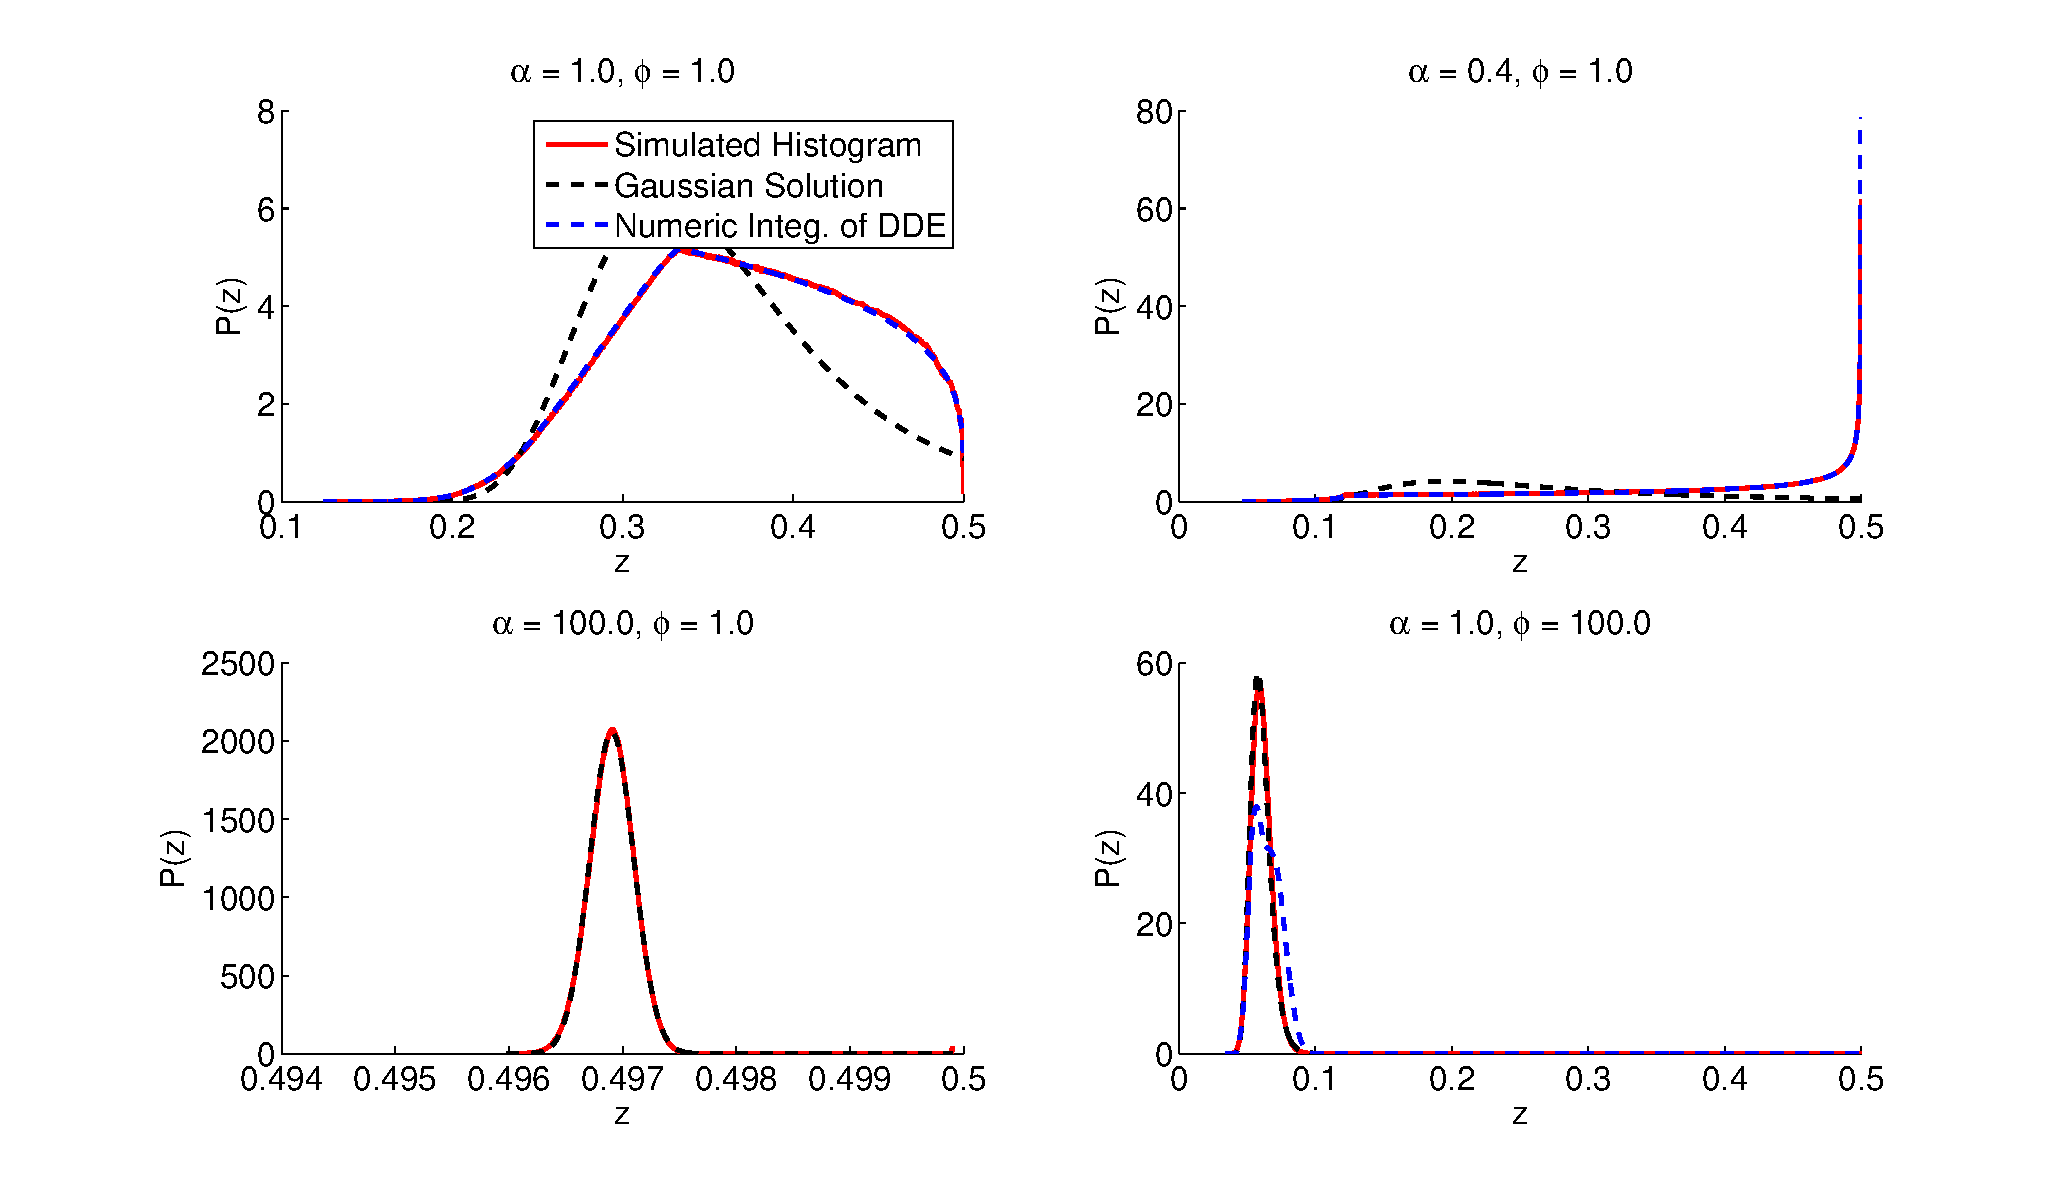
\includegraphics[width=\columnwidth]{figures/solution_comparison_OU.eps}
\caption{The two approaches to solving for the equilibrium distribution described, shown across a range of parameter values.}
\end{figure}
One particularly interesting characteristic of this solution is the exponent. Note that the sign of the exponent in \fref{eq:dist_1d_exact} depends on the specific value of $\hat{\lambda}$ and $2\gamma$. If $\hat{\lambda} > 2\gamma$, the exponent will be larger than 0, leading the distribution to tend to $0$ as $s$ tends to $s_0$. If, however, $\hat{\lambda} < 2\gamma$, the exponent will be negative, leading the distribution to diverge around $s_0$. Notice that $s_0$ is the worst possible performance our encoder can achieve, as it is the variance of the unobserved process. This tells us that whenever the firing rate of the population is below a certain value, the probability distribution of our MSE will be concentrated around its worst possible value. These results are nicely illustrated in \fref{fig:comparison_histograms} where we provide histograms of the exact solution, numerical simulations and a Gaussian approximation to the distribution. This is very interesting, as it relates two different time scales, one ($1/2\gamma$) defines how long information about the observed process stays relevant, while the other ($1/\hat{\lambda}$) given the average time between observations. This provides a rigorous interpretation of an intuitive property of temporal estimation schemes.
\par
Note that, although this result is always valid in the interval $S_0$, we can derive it in the limit of low firing rates as well. If we assume the population firing rate $\hat{\lambda} \ll 2\gamma$, then we will find that the expected interspike interval is much longer than the characteristic time of the variance's dynamics. It is then safe to assume, that whenever a spike is fired, the variance is very close to its equilibrium value $s_0 = \sigma/2\gamma$. The evolution of it after the spike time $t_s$ will then be given by
\[
s(t) = e^{-2\gamma(t-t_s)} s' + s_0 \left(1-e^{-2\gamma (t-t_s)}\right),
\]
where $s' = j(s_0)$,
We can promptly isolate the time in this equation to obtain
\[
\tau \equiv (t-t_s) = -\frac{1}{2\gamma} \log\left(\frac{s_0-s(t)}{s_0-s'}\right).
\]
Clearly, if the spikes are sampled from a Poisson process, then the interspike intervals have a exponential distribution and we will have $P(\tau) \propto e^{-\hat{\lambda}\tau}$. Through a change of variables we then obtain
\[
P(s) = P(\tau) \left|\frac{d\tau}{ds}\right| \propto e^{-\hat{\lambda} \tau + 2\gamma \tau}.
\]
Inserting the definition for $\tau$ we will recover \fref{eq:dist_1d_exact}. Note that this is an approximation for $P(s)$ throughout the range of $s$ for a particular parameter limit, whereas before we had derived an exact result for any parameters, but limited to a small range of values of $s$.\par
We can derive a similar limit for the multidimensional case. Let us first assume $\hat{\lambda}$ is small enough for the covariance $s$ to have relaxed to its equilibrium value $s_0$. After a spike the covariance is then given by $s' = \left(s_0^{-1}+A^\dagger\right)^{-1}$. The evolution of $s(t)$ after a spike at $t_s$ is then given by
\[
s(\tau) = e^{\tau G} s' e^{\tau G^\top} + \int_0^\tau e^{\tau G}\sigma e^{\tau G^\top}.
\]
We could in principle proceed as before, but the mapping from the matrix space to the one-dimensional time space can not be explicitly written as above. One alternative is to evaluate the marginals of the diagonal entries of the covariance matrix numerically. We will have, as before,
\[
P(s_{11}) = \frac{P(\tau(s_{11}))}{\left|\frac{d s_{11}}{d\tau}\right|} \propto \frac{e^{-\hat{\lambda} \tau}}{\left|\frac{d s_{11}}{d\tau}\right|}.
\]
We can then evaluate the derivative numerically and obtain an estimate of the distribution of $s_{11}$. If $G$ introduces interactions between the entries of the covariance matrix, however, this result will not prove as powerful, though. As an example, we can consider the Matern processes considered in \citep{Susemihl2012a}, where we have $ds_{11}/dt = s_12$. But immediately after the jump, $s'_{12} = 0$, leading the distribution to diverge at $s'_{11}$ as well as in $s^0_{11}$. So, although the divergence around the equilibrium covariance remains, further divergences introduced by the matrix $G$ will reduce the impact of $\hat{\lambda}$ on the shape of the distribution. An example is shown in \fref{fig:matern_histograms}.
\begin{figure}
\label{fig:matern_histograms}
\includegraphics[width=\columnwidth]{figures/matern_histogram.eps}
\caption{The small firing rate limit for the Matern process.}
\end{figure}
\subsection{Van Kampen Approximation}


